\documentclass[20pt,landscape,dvips]{foils} 
% add 'draft' option above to exclude image when compiling
\usepackage[french]{babel}
\usepackage[utf8]{inputenc}  
\usepackage{csquotes} 
%\MakeOuterQuote{"}
\frenchspacing
\DecimalMathComma

\usepackage{latexsym}
\usepackage{amsmath,amssymb,amsfonts}
\usepackage{MnSymbol}
\usepackage{url}
\usepackage{graphicx}
%\usepackage[dvipsnames]{xcolor}
\usepackage{hyperref}
\usepackage{alltt}
\usepackage{pifont,manfnt}
\usepackage[dvipsnames,table]{xcolor}
\usepackage{subfig}
%\usepackage{enumerate}
%\usepackage{colortbl}
\usepackage{multirow,hhline}
\usepackage{cclicenses}
\setlength\parindent{0pt}
\hypersetup{colorlinks=true,citecolor=black,urlcolor=black,linkcolor=black}
\usepackage[style=verbose]{biblatex}
\bibliography{refs}

\newcommand{\highlight}[1]{\textcolor{Plum}{\bfseries #1}}
\newcommand{\remark}[1]{%
%\centerline{
\begin{center}
\framebox[.9\textwidth][t]{
\ding{46} 
\parbox[t]{.8\textwidth}{\small #1}}
\end{center}}

\DeclareMathOperator*{\inlaw}{\sim}
\newcommand{\iid}{\inlaw_{\text{i.i.d.}}}
%\newcommand{\iid}{\mathop{\mathrm{diag}}}
\newcommand{\pobs}{p_{\text{obs}}}

\reversemarginpar
\def\mark{\marginpar{\dbend}}

%\newcommand{\bm}[1]{\mbox{\boldmath{$#1$}}}
\renewcommand{\abstractname}{Summary}
\newcommand\bs{\char '134}   %  a backslash character for the \tt font
%\renewcommand\refname{Additional Readings}

% customize header/footer
\rightheader{}
% Note about the copyleft symbol:
% I use a custom reversed and circled "c" char because \textcopyleft in
% the textcomp package does not support sans serif font.
% Also, "c" is shifted horizontally by 1ex to align with the circle.
%\Restriction{\mbox{\raisebox{1.5ex}{\rotatebox{180}{\textcircled{c\kern.1ex}}} 2009}, \url{www.aliquote.org}}
% now I use the CC licence...
% \Restriction{\cc 2016 \VCRevision}
\Restriction{\cc 2016 Module 11 EESPE}

\title{Méthodes psychométriques en qualité de vie}
\author{Christophe Lalanne\\EA 7334 REMES\\ Unité de Méthodologie des critères d’évaluation\\Université Paris-Diderot, Sorbonne Paris-Cité\\}
\date{
\includegraphics[height=18ex]{logo.eps}}

%%% This file has been generated by the vc bundle for TeX.
%%% Do not edit this file!
%%%
%%% Define Git specific macros.
\gdef\GITHash{f4328f7906d309e9224e3e5c2f7f36477f44e69f}%
\gdef\GITAbrHash{f4328f7}%
\gdef\GITParentHashes{136657e4877819e72dc9ebb2f209631a2a8d1057}%
\gdef\GITAbrParentHashes{136657e}%
\gdef\GITAuthorName{Christophe Lalanne}%
\gdef\GITAuthorEmail{ch.lalanne@gmail.com}%
\gdef\GITAuthorDate{2016-07-06 10:29:58 +0200}%
\gdef\GITCommitterName{Christophe Lalanne}%
\gdef\GITCommitterEmail{ch.lalanne@gmail.com}%
\gdef\GITCommitterDate{2016-07-06 10:29:58 +0200}%
%%% Define generic version control macros.
\gdef\VCRevision{\GITAbrHash}%
\gdef\VCAuthor{\GITAuthorName}%
\gdef\VCDateRAW{2016-07-06}%
\gdef\VCDateISO{2016-07-06}%
\gdef\VCDateTEX{2016/07/06}%
\gdef\VCTime{10:29:58 +0200}%
\gdef\VCModifiedText{\textcolor{red}{with local modifications!}}%
%%% Assume clean working copy.
\gdef\VCModified{0}%
\gdef\VCRevisionMod{\VCRevision}%


\begin{document}
\LogoOff
\maketitle
\rightfooter{\quad\textsf{\thepage}}



%---------------------------------------------------------------Slide-
\foilhead{Analyses factorielles}
\begin{itemize}
\item Analyse en composantes principales et analyse factorielle
\item Analyse factorielle exploratoire
\item Analyse factorielle confirmatoire
\end{itemize}


% ---------------------------------------------------------------Slide-
\foilhead{}

\begin{quote}
It is rather surprising that systematic studies of human abilities were not undertaken until the second half of the last century\ldots An accurate method was available for measuring the circumference of the earth 2,000 years before the first systematic measures of human ability were developed\autocite{Nunnally1994}.  
\end{quote}

% ---------------------------------------------------------------Slide-
\foilhead{Avant Jan de Leeuw \& Bengt Muthén}

{\centering \fbox{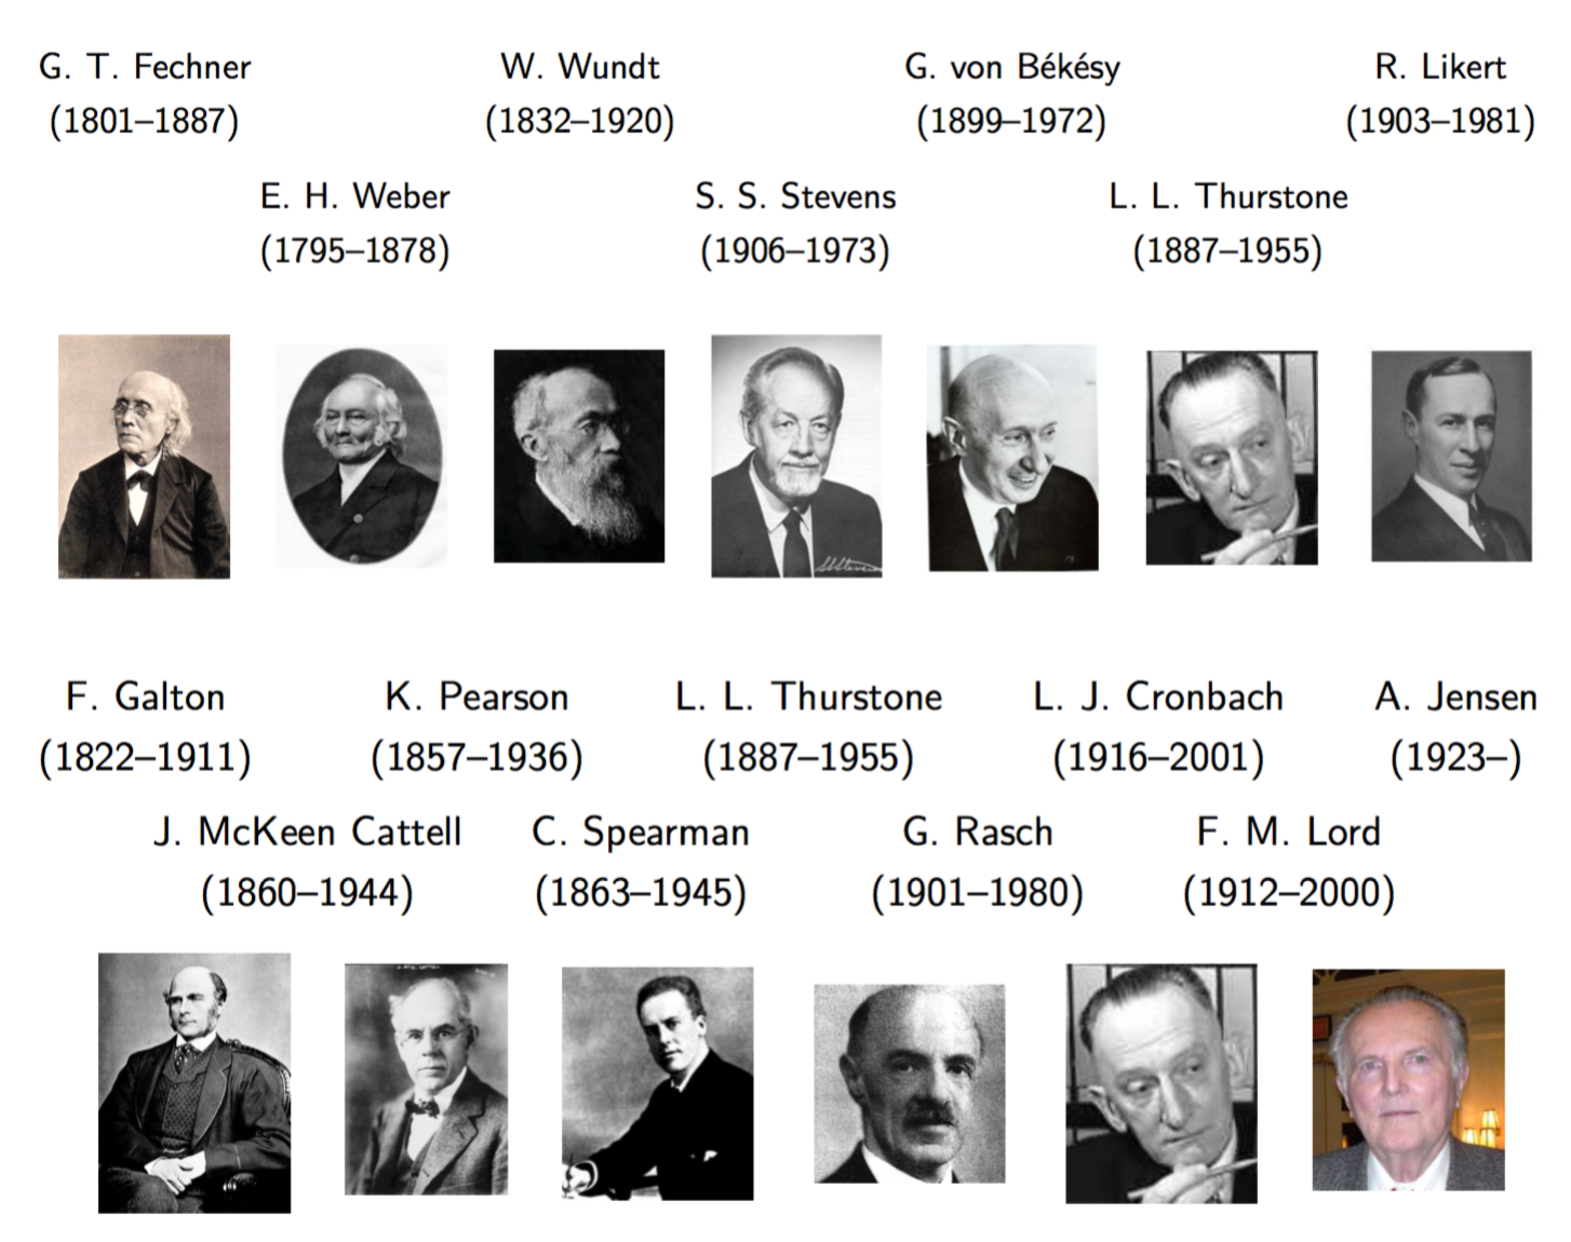
\includegraphics[width=.6\textwidth]{figs/history.eps}}\par}

% ---------------------------------------------------------------Slide-
\foilhead{}

{\centering \fbox{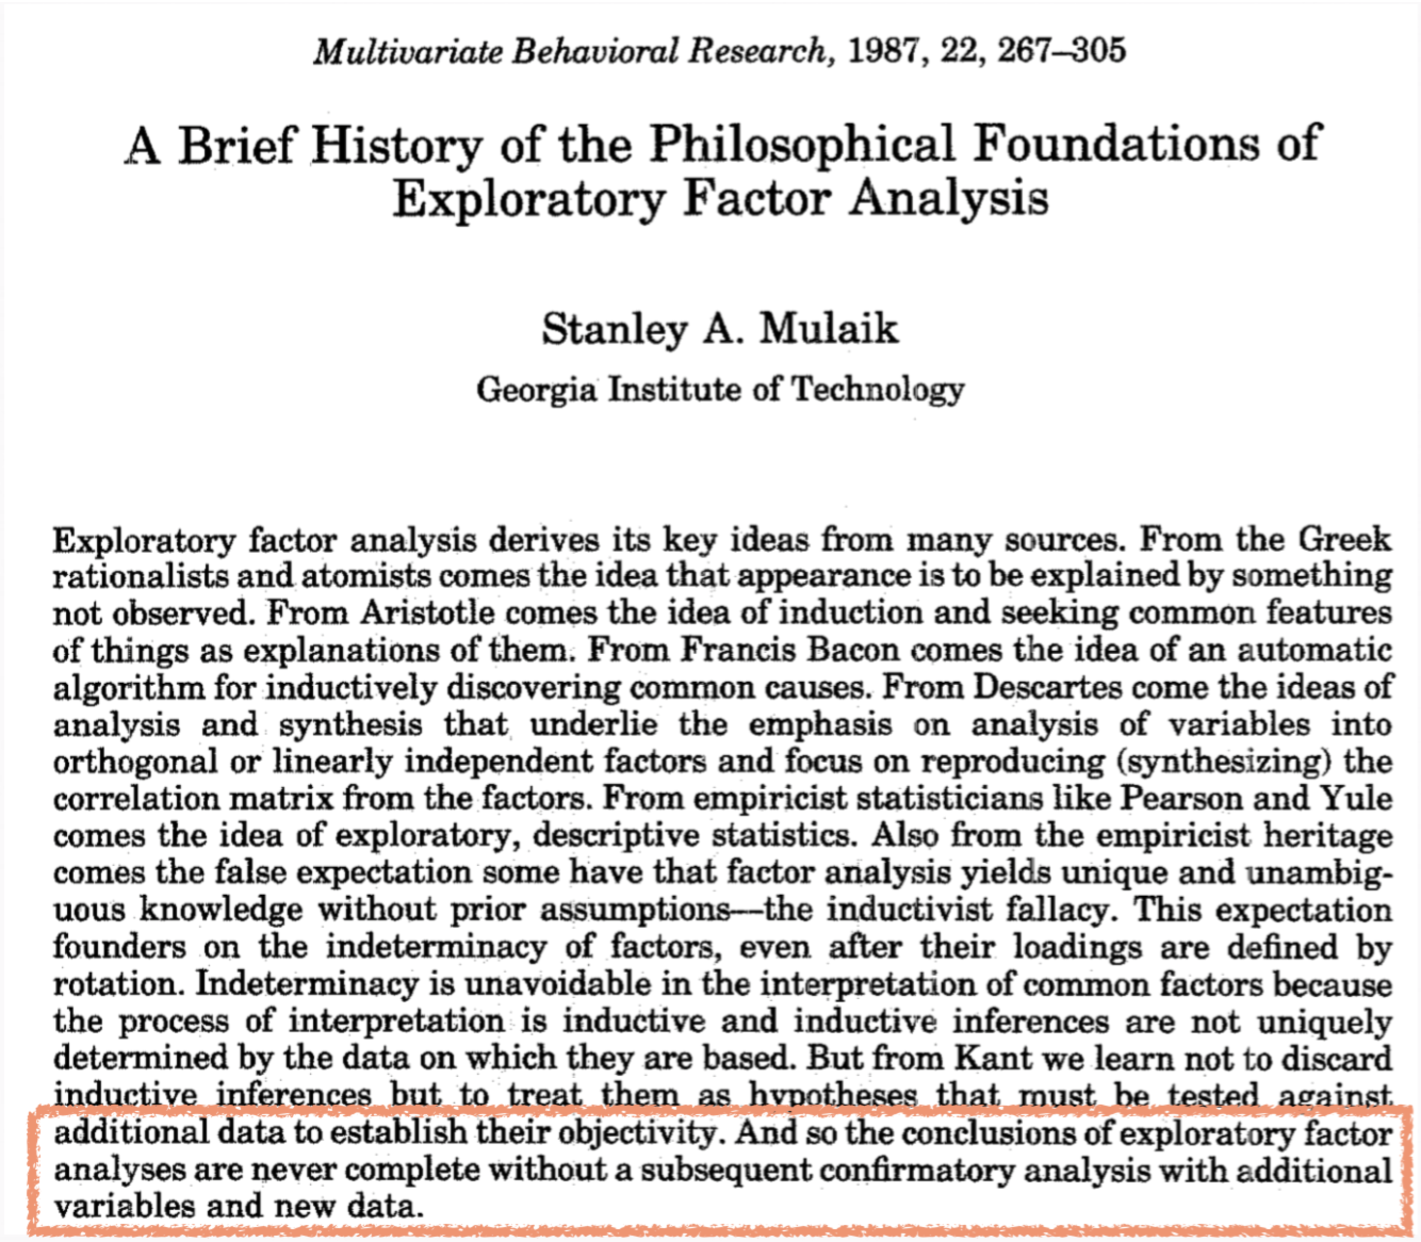
\includegraphics[width=.6\textwidth]{figs/efa.eps}}\par}


% ---------------------------------------------------------------Slide-
\foilhead{ACP et AF}
\hfill $\triangleright$ 01a-scores.pdf

Les composantes $C_i$ ($i=1,\dots,p$) de l'analyse en composantes principales
(ACP) sont construites comme de simples combinaisons linéaires des $p$ variables
d'origine : $C_i=\sum_{j=1}^pw_{ij}\textcolor{Apricot}{x_j}$.

Dans le cadre de l'analyse factorielle, on considère au contraire des
combinaisons linéaires de facteurs\autocite[chap.~ 6]{revelle16} :
\[
\textcolor{Apricot}{x_i}\approx\sum_{j=1}^kw_{ij}\textcolor{CornflowerBlue}{F_j}.
\]


% ---------------------------------------------------------------Slide-
\foilhead{Modèle de Holzinger \& Swineford}

{\centering \fbox{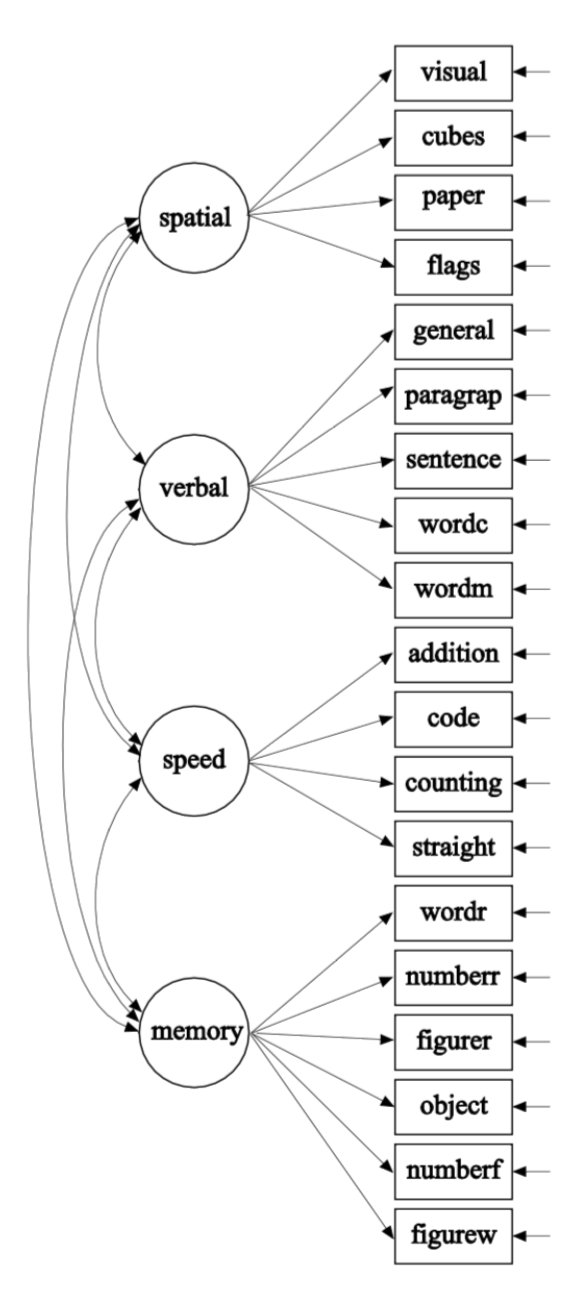
\includegraphics[width=.35\textheight]{figs/HS2.eps}}\par}


% ---------------------------------------------------------------Slide-
\foilhead{Comparaison ACP \emph{versus} AF}

\begin{alltt}
library(psych)
principal(HS[,c("visual","cubes", paper")], \highlight{nfactors = 3}, 
          rotate = "none")
\end{alltt}
\begin{alltt}\small
Standardized loadings (pattern matrix) based upon correlation matrix
        PC1   PC2   PC3 h2       u2 com
visual 0.77 -0.41  0.48  1  0.0e+00 2.3
cubes  0.70  0.71  0.10  1 -4.4e-16 2.0 \ding{182}
paper  0.80 -0.22 -0.56  1 -6.7e-16 2.0

                       PC1  PC2  PC3
SS loadings           1.72 0.72 0.56
Proportion Var        0.57 0.24 0.19
\end{alltt}

% ---------------------------------------------------------------Slide-
\foilhead{}

\begin{alltt}
fa(HS[,c("visual", "cubes", "paper")], nfactors = 1)
\end{alltt}
\begin{alltt}\small
Standardized loadings (pattern matrix) based upon correlation matrix
        MR1   h2   u2 com
visual 0.62 0.39 0.61   1
cubes  0.48 0.23 0.77   1 \ding{182}
paper  0.71 0.50 0.50   1

                MR1
SS loadings    1.12
Proportion Var 0.37
\end{alltt}

% ---------------------------------------------------------------Slide-
\foilhead{Sélection de modèle}
\begin{itemize}
\item Sélection des variables à inclure : analyse d'items ou hypothèses \emph{a
    priori}
\item Sélection du nombre de facteurs : méthode exploratoire, hypothèses \emph{a
    priori}, analyse parallèle \autocite{humphreys75}
\item Type de rotation : en fonction des hypothèses théoriques
\item Méthode d'estimation (OLS, ML, WLS et PA)
\item Matrice de corrélation (Pearson, tétra- ou polychorique)  
\item Nombre de sujets nécessaires \autocite{rouquette11}
\end{itemize}


% ---------------------------------------------------------------Slide-
\foilhead{Analyse parallèle}

\begin{alltt}
d <- HS[,7:15]
describe(d)
fa.parallel(d, fm = "pa", fa = "fa", main = "")
\end{alltt}

{\centering 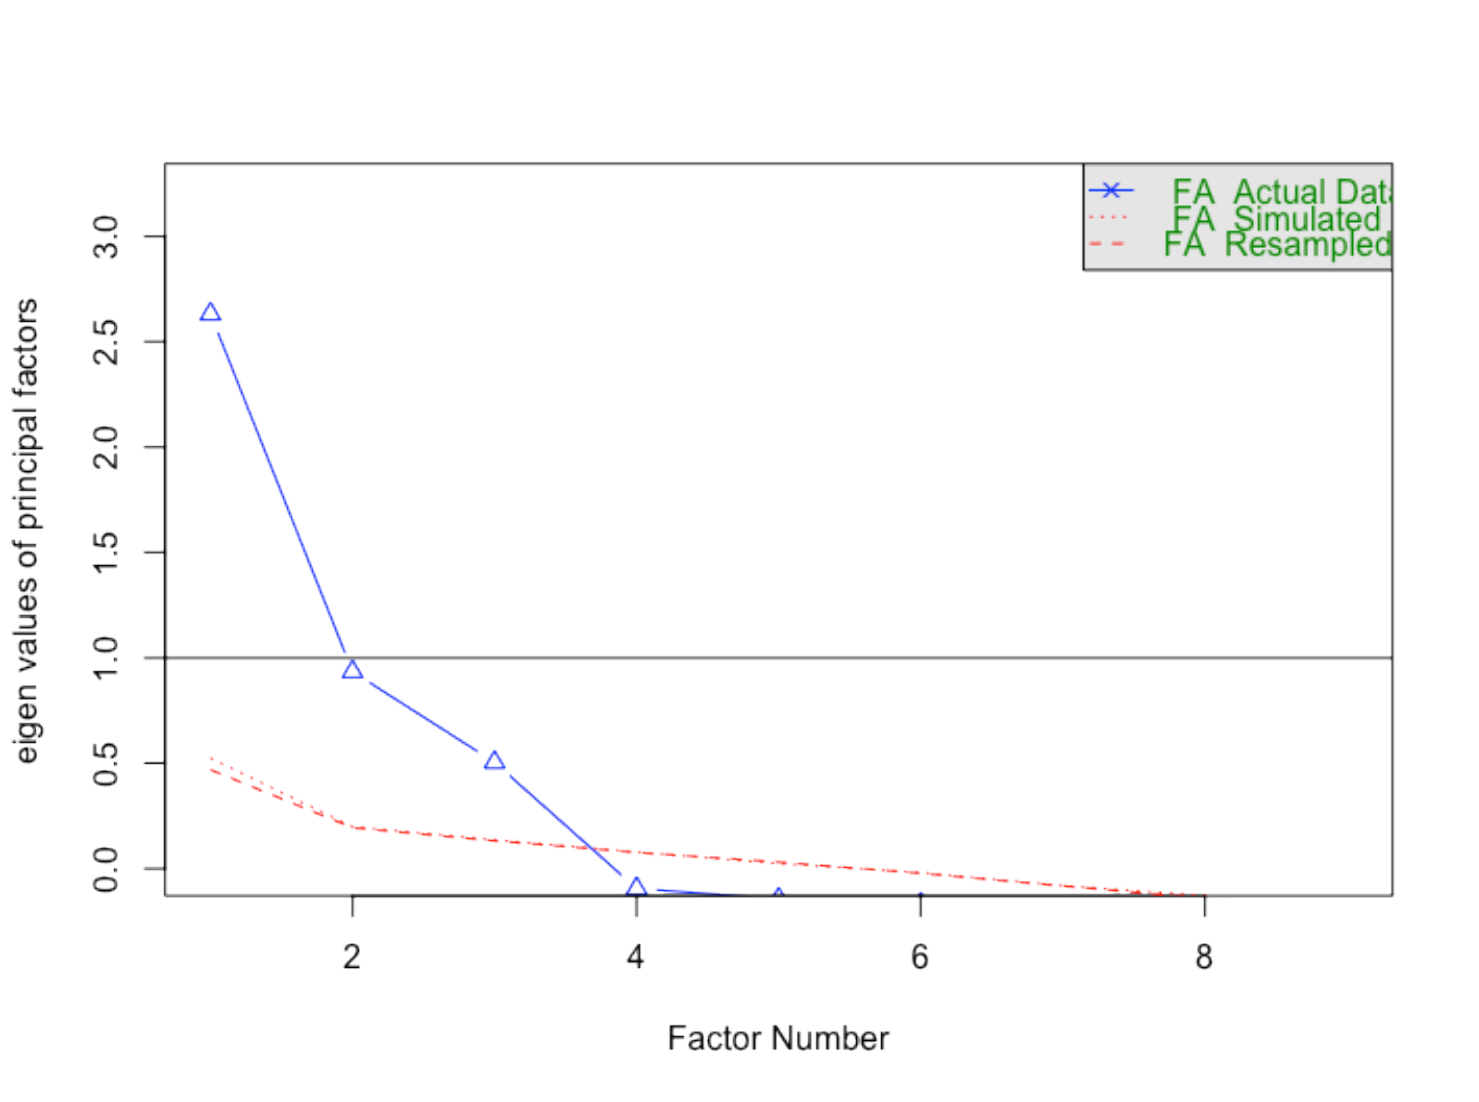
\includegraphics[width=.4\textwidth]{figs/p26.eps}\par}


% ---------------------------------------------------------------Slide-
\foilhead{Solution factorielle à 1 facteur}

{\centering 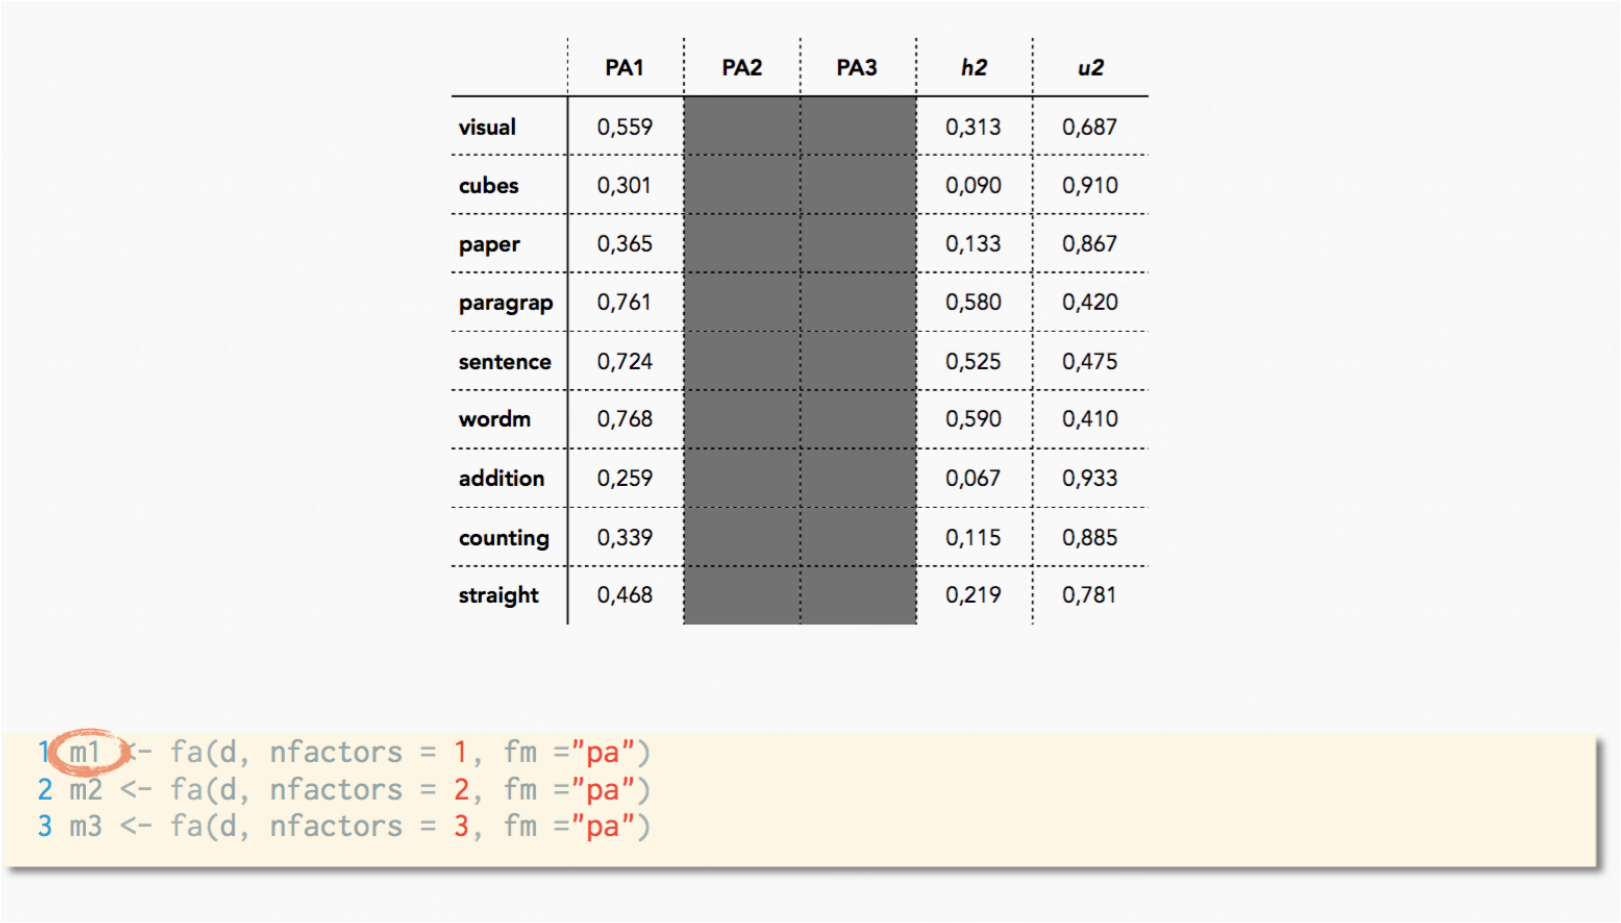
\includegraphics[width=.8\textwidth]{figs/sol1.eps}\par}

% ---------------------------------------------------------------Slide-
\foilhead{Solution factorielle à 2 facteurs}

{\centering 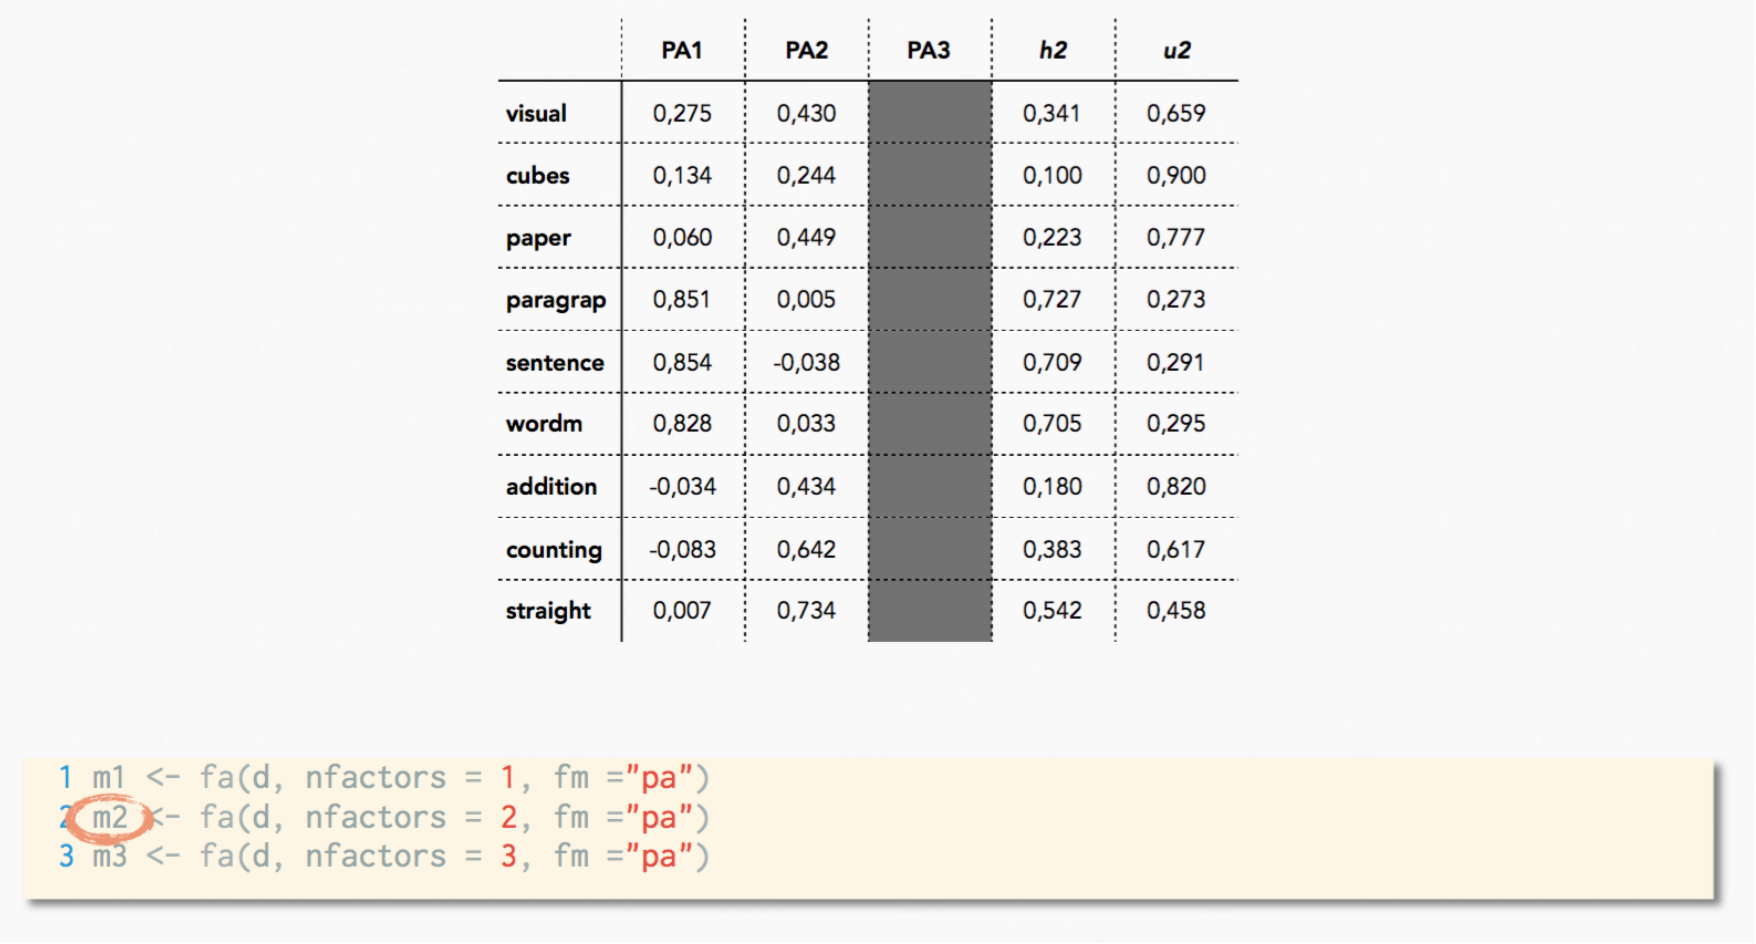
\includegraphics[width=.8\textwidth]{figs/sol2.eps}\par}

% ---------------------------------------------------------------Slide-
\foilhead{Solution factorielle à 3 facteurs}

{\centering 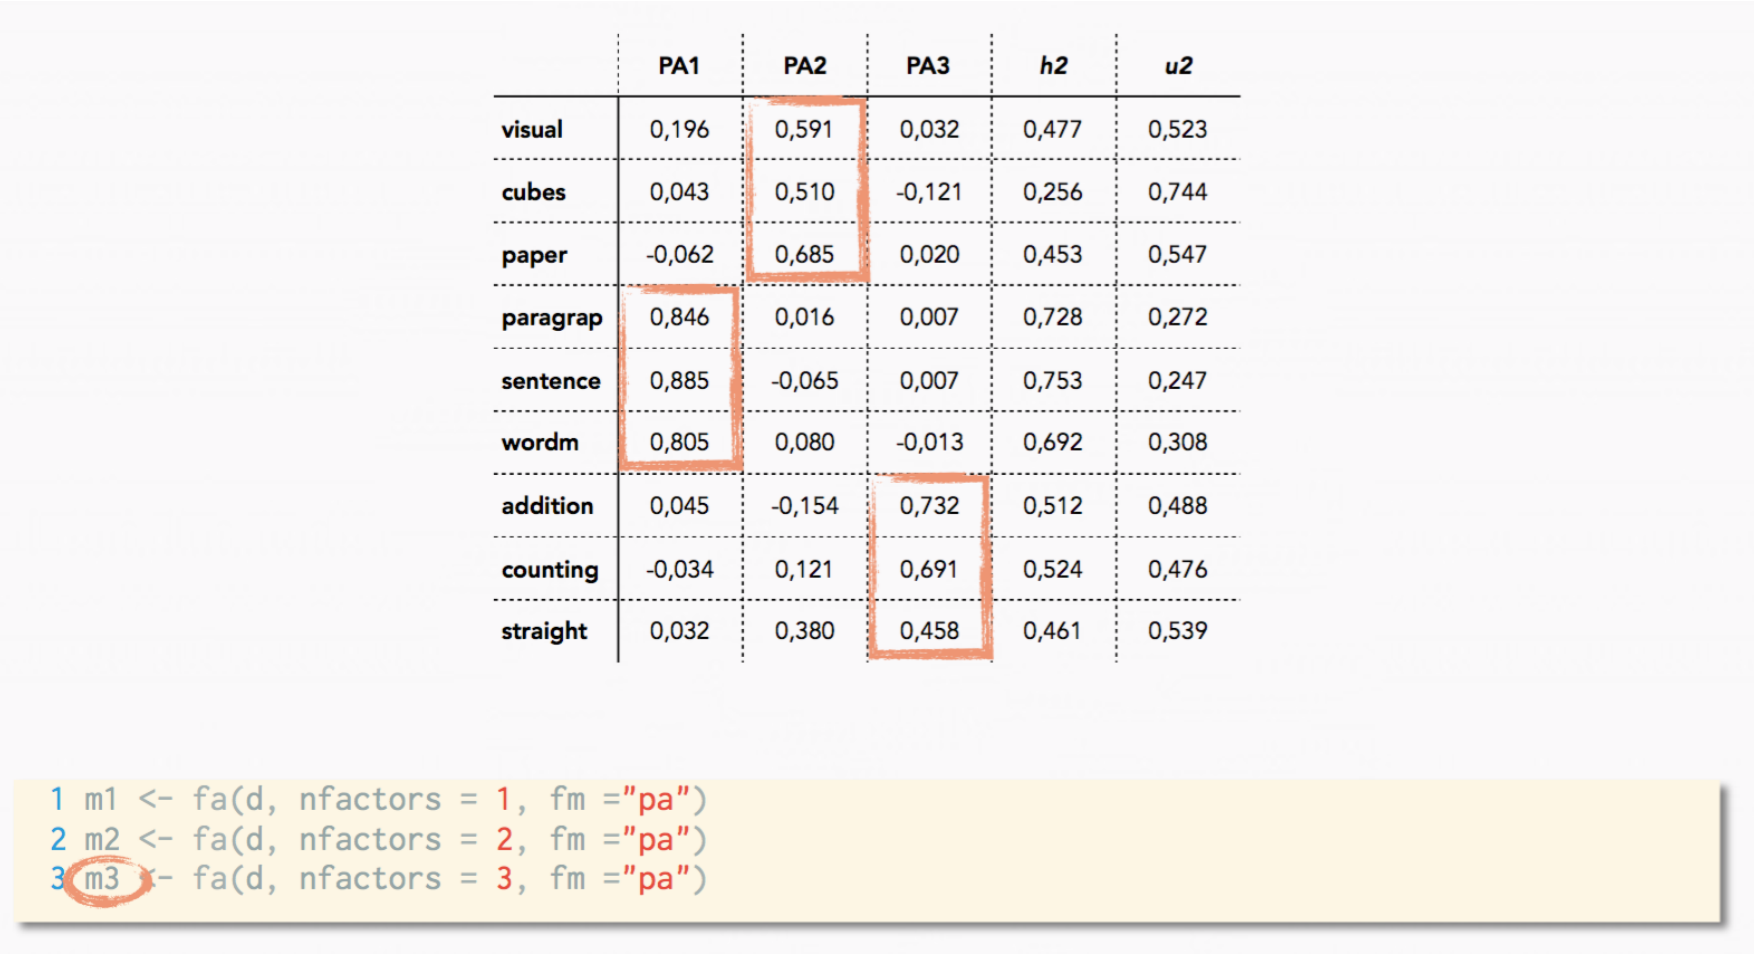
\includegraphics[width=.8\textwidth]{figs/sol3.eps}\par}


% ---------------------------------------------------------------Slide-
\foilhead{Analyse exploratoire et confirmatoire (CFA)\autocite{Jackson2009,hu99}}

\begin{minipage}{0.45\textwidth}
La CFA revient à imposer une structure particulière, c.a.d. à contraindre certains
paramètres du modèle, et à tester l'adéquation du modèle avec les données.
\end{minipage}\hfill
\begin{minipage}{0.5\textwidth}
\centerline{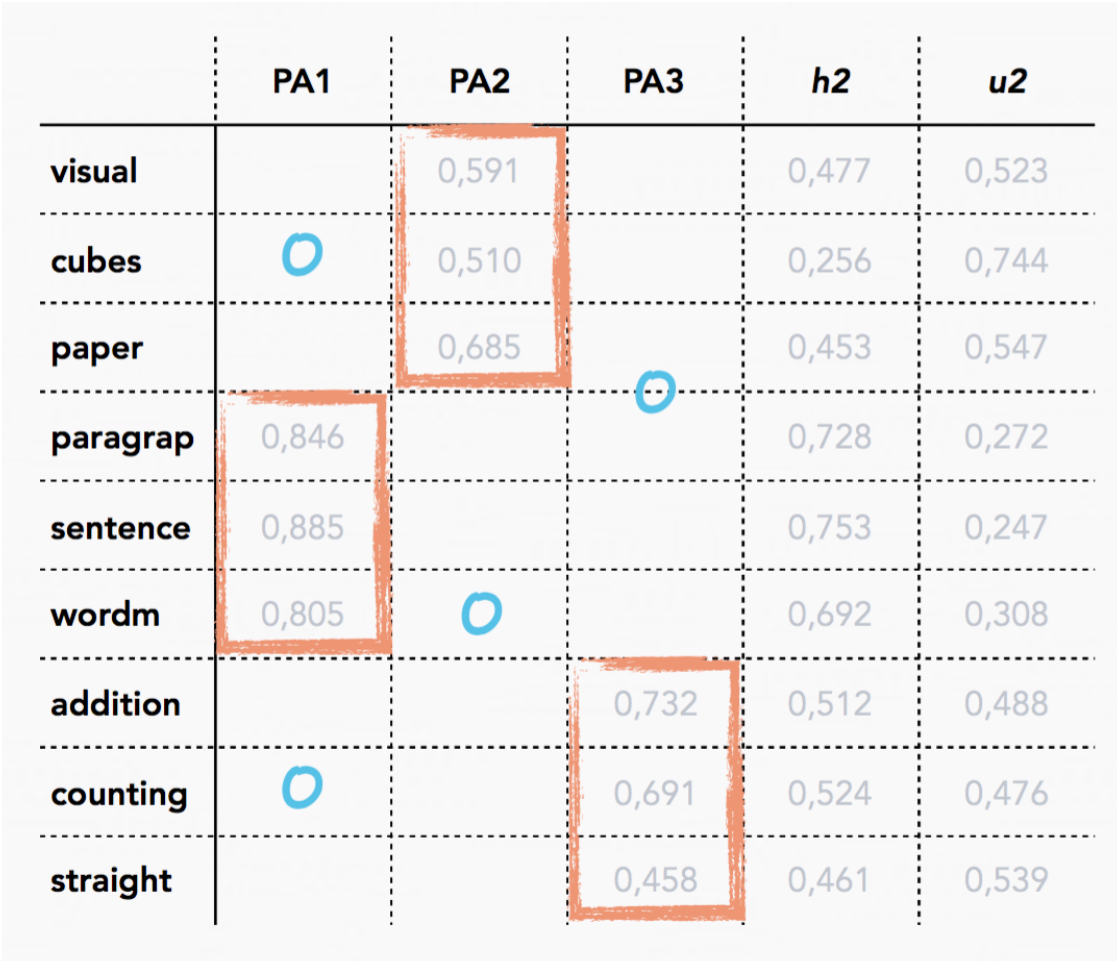
\includegraphics[scale=.5]{./figs/cfa.eps}}
\end{minipage}


% ---------------------------------------------------------------Slide-
\foilhead{Utilisation de \texttt{lavaan}}
Le package \texttt{lavaan}\autocite{rosseel12} dispose de 4 commandes essentielles :
\texttt{lavaan}, \texttt{cfa}, \texttt{sem}, \texttt{growth}.

Les commandes inclut entre autres des procédures d'estimation par intervalles
(bootstrap), de simulation et de transfert de données/modèles avec
Mplus\autocite{beaujean13,beaujean14}.

{\centering \url{http://lavaan.ugent.be}\par}


% ---------------------------------------------------------------Slide-
\foilhead{Modèle en traits corrélés}

\begin{alltt}
library(lavaan)
library(semPlot)
m <- 'Visual =~ visual + cubes + paper \hfill \ding{182}
      Verbal =~ paragrap + sentence + wordm
      Speed  =~ addition + counting + straight'
r <- cfa(m, data = d) \hfill \ding{183}
summary(r, fit.measures = TRUE) \hfill \ding{184}
semPaths(r, whatLabels = "est") \hfill \ding{185}
\end{alltt}
\begin{alltt}\small
> summary(r, fit.measures = TRUE)
lavaan (0.5-20) converged normally after  35 iterations

  Number of observations                           301

  Estimator                                         ML
  Minimum Function Test Statistic               85.306
  Degrees of freedom                                24
  P-value (Chi-square)                           0.000

Model test baseline model:

  Minimum Function Test Statistic              918.852
  Degrees of freedom                                36
  P-value                                        0.000

User model versus baseline model:

  Comparative Fit Index (CFI)                    0.931 \hfill \ding{182}
  Tucker-Lewis Index (TLI)                       0.896

Loglikelihood and Information Criteria:

  Loglikelihood user model (H0)              -3737.745
  Loglikelihood unrestricted model (H1)      -3695.092

  Number of free parameters                         21
  Akaike (AIC)                                7517.490
  Bayesian (BIC)                              7595.339
  Sample-size adjusted Bayesian (BIC)         7528.739

Root Mean Square Error of Approximation:

  RMSEA                                          0.092 \hfill \ding{183}
  90 Percent Confidence Interval          0.071  0.114
  P-value RMSEA <= 0.05                          0.001

Standardized Root Mean Square Residual:

  SRMR                                           0.065 \hfill \ding{184}

Parameter Estimates:

  Information                                 Expected
  Standard Errors                             Standard

Latent Variables:
                   Estimate  Std.Err  Z-value  P(>|z|)
  Visual =~
    visual            1.000  \hfill \ding{185}
    cubes             0.554    0.100    5.554    0.000
    paper             0.729    0.109    6.685    0.000
  Verbal =~
    paragrap          1.000
    sentence          1.113    0.065   17.014    0.000
    wordm             0.926    0.055   16.703    0.000
  Speed =~
    addition          1.000
    counting          1.180    0.165    7.152    0.000
    straight          1.082    0.151    7.155    0.000

Covariances:
                   Estimate  Std.Err  Z-value  P(>|z|)
  Visual ~~
    Verbal            0.408    0.074    5.552    0.000 \hfill \ding{186}
    Speed             0.262    0.056    4.660    0.000
  Verbal ~~
    Speed             0.173    0.049    3.518    0.000

Variances:
                   Estimate  Std.Err  Z-value  P(>|z|)
    visual            0.549    0.114    4.833    0.000
    cubes             1.134    0.102   11.146    0.000
    paper             0.844    0.091    9.317    0.000
    paragrap          0.371    0.048    7.779    0.000
    sentence          0.446    0.058    7.642    0.000
    wordm             0.356    0.043    8.277    0.000
    addition          0.799    0.081    9.823    0.000
    counting          0.488    0.074    6.573    0.000
    straight          0.566    0.071    8.003    0.000
    Visual            0.809    0.145    5.564    0.000
    Verbal            0.979    0.112    8.737    0.000
    Speed             0.384    0.086    4.451    0.000
\end{alltt}


% ---------------------------------------------------------------Slide-
\foilhead{Modèle en traits corrélés (paramétrisation alternative)}

\begin{alltt}
r <- cfa(m, data = d, \highlight{std.lv = TRUE}) 
\end{alltt}


{\centering 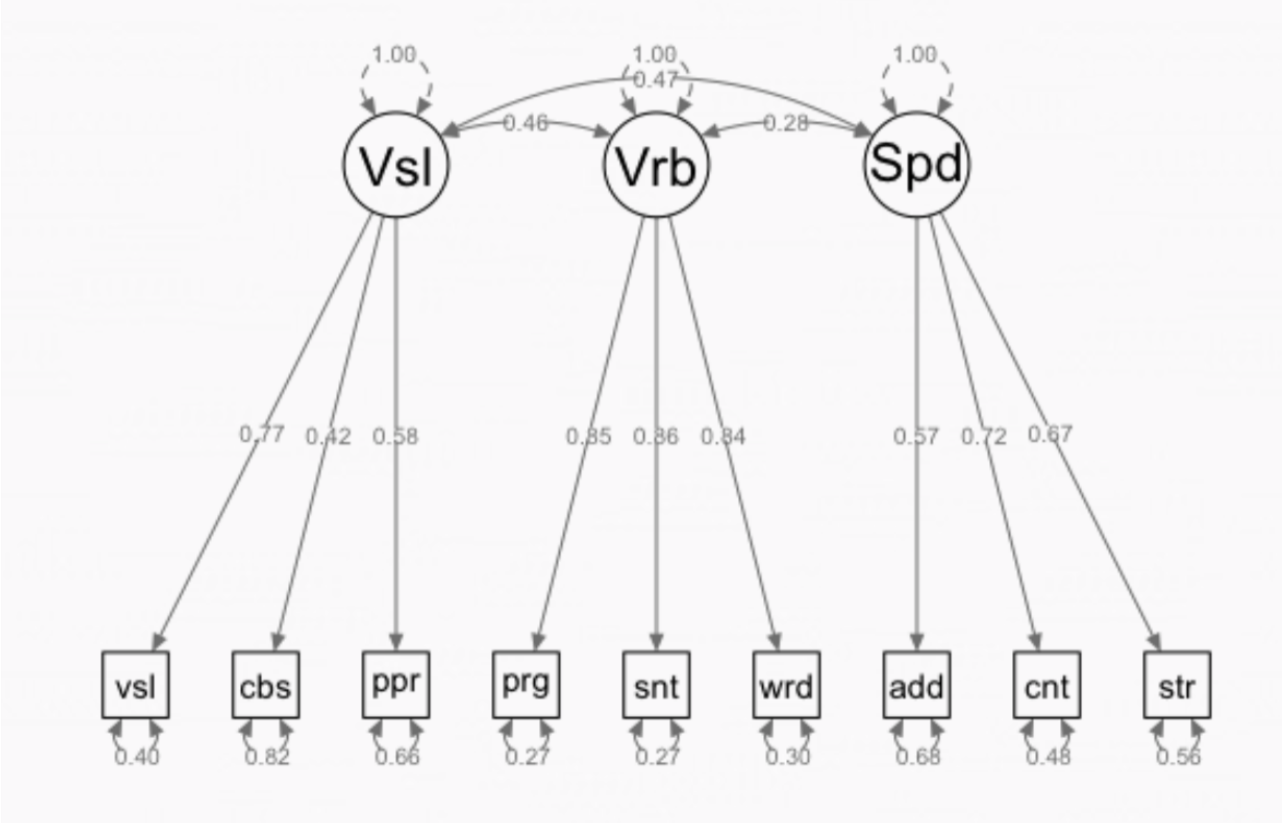
\includegraphics[width=.6\textwidth]{figs/m2.eps}\par}

% ---------------------------------------------------------------Slide-
\foilhead{Modèle en traits orthogonaux}

\begin{alltt}
r <- cfa(m, data = d, \highlight{orthogonal = TRUE}) 
\end{alltt}

{\centering 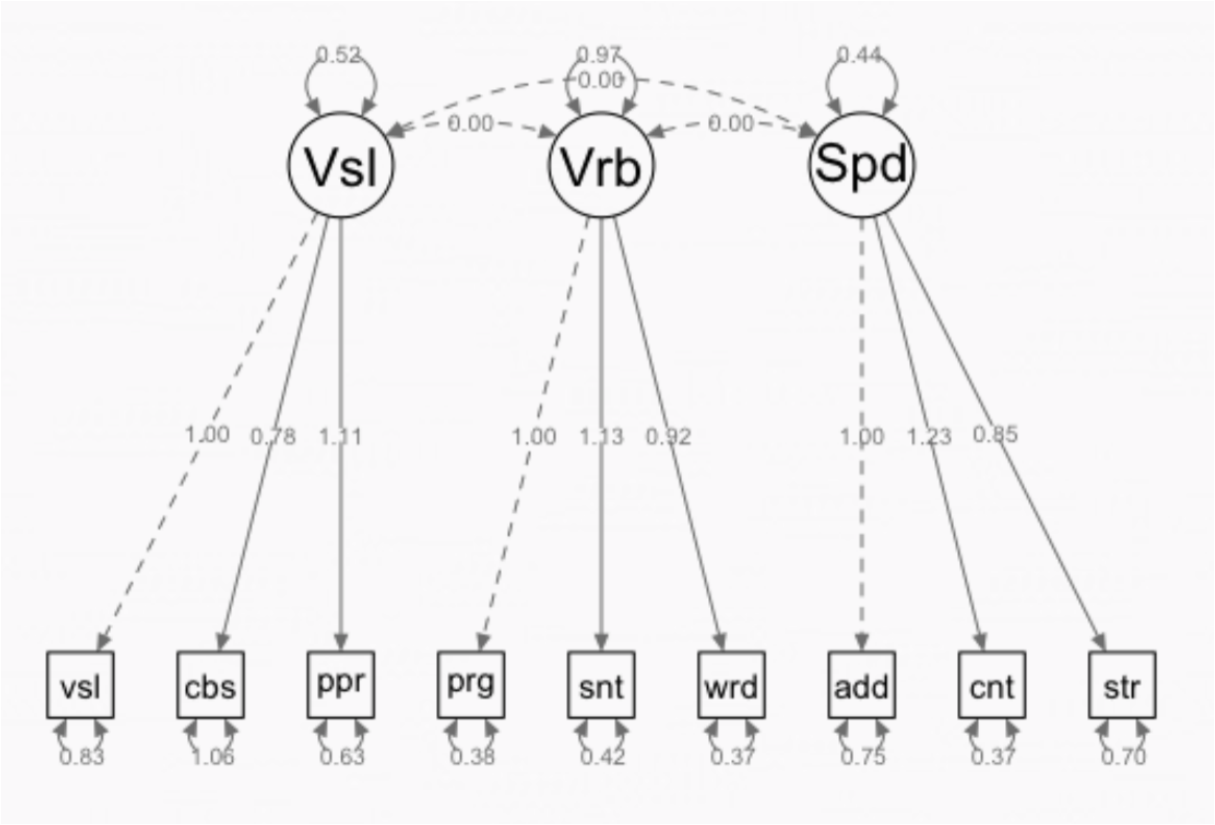
\includegraphics[width=.6\textwidth]{figs/m3.eps}\par}


% ---------------------------------------------------------------Slide-
\foilhead{Modèles de mesure en analyse factorielle}

{\centering \fbox{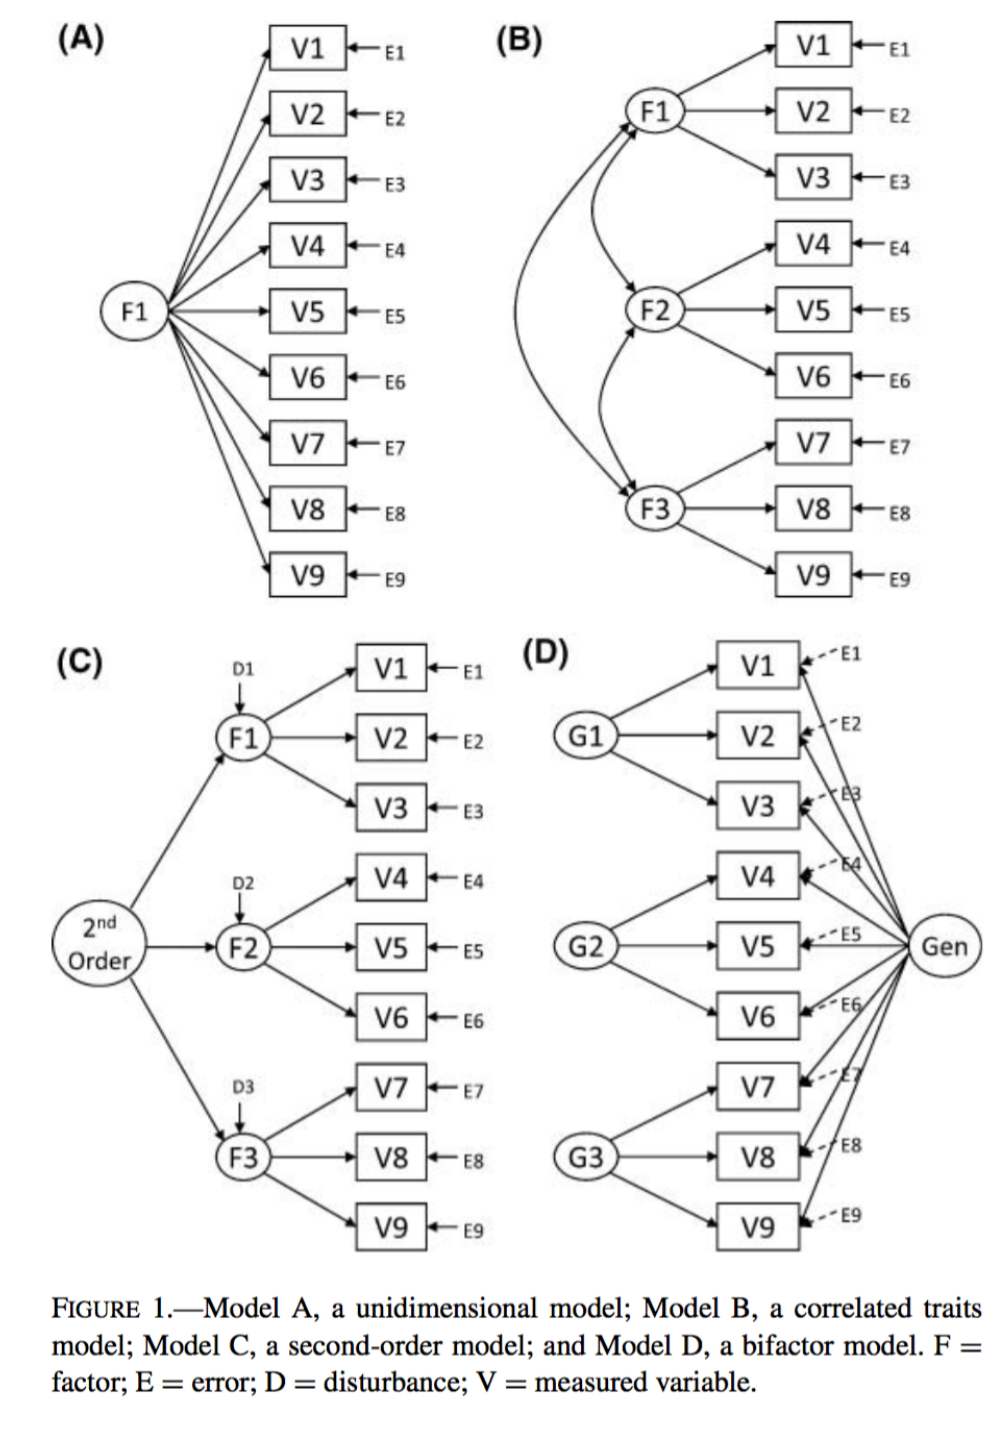
\includegraphics[width=.55\textheight]{figs/models.eps}}\par}


% ---------------------------------------------------------------Slide-
\foilhead{Modèles alternatifs pour les données HS}

\begin{itemize}
\item \highlight{Modèle de second ordre} : modèle de mesure placé directement au
  niveau de la corrélation entre les facteurs spécifiques : les facteurs sont
  corrélés car ils \enquote{partagent une cause commune}. L'effet facteur
  primaire est appelé effet indirect.
\item \highlight{Modèle bifactoriel} : tous les items sont associés à un même
  facteur général, et ce modèle inclut des facteurs spécifiques orthogonaux,
  appelés facteurs communs, qui résument la variance non expliquée par le
  facteur général \autocite{reise10}.
\end{itemize}

% ---------------------------------------------------------------Slide-
\foilhead{Modèle de second ordre}

\begin{alltt}
m3 <- 'Visual =~ visual + cubes + paper
       Verbal =~ paragrap + sentence + wordm
       Speed  =~ addition + counting + straight
       F =~ Visual + Verbal + Speed'
\end{alltt}

{\centering 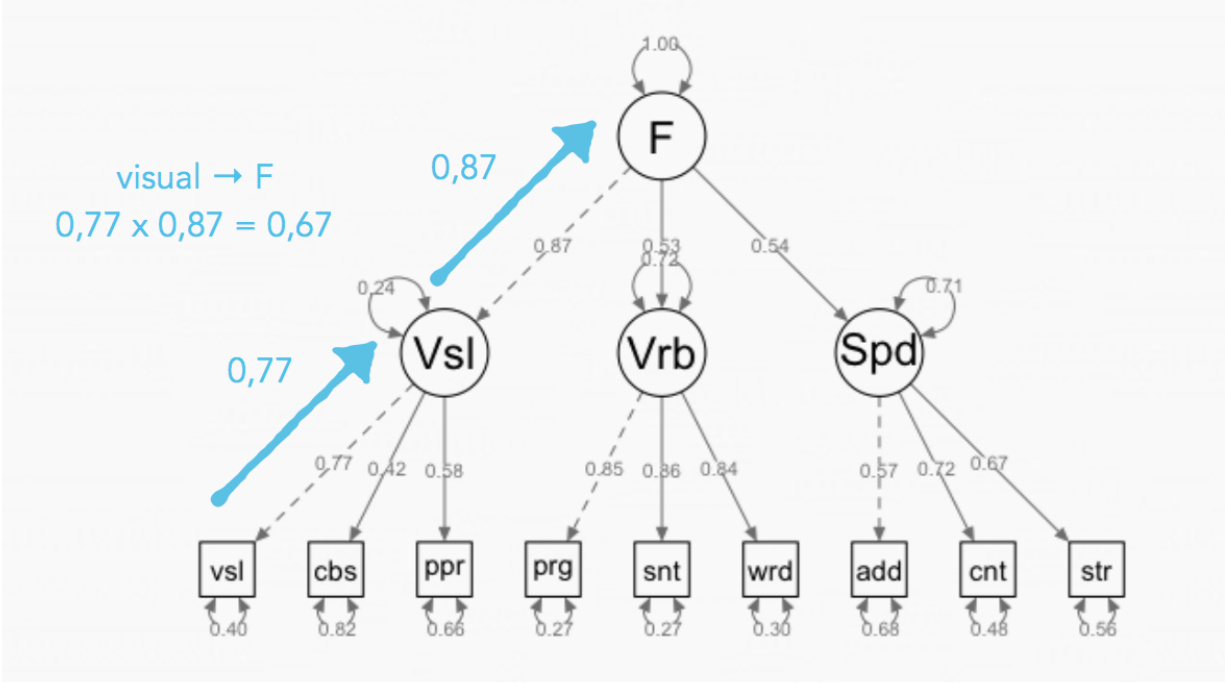
\includegraphics[width=.5\textwidth]{figs/m4.eps}\par}

% ---------------------------------------------------------------Slide-
\foilhead{Applications}

\begin{enumerate}
\item Refaire l'analyse CFA séparément dans les deux groupes définis par la
  variable \texttt{school} et comparer les charges factorielles entre les deux
  échantillons.
\item À partir des données \texttt{HADS.RData} \autocite{bartolucci16}, réaliser
  une analyse d'items et vérifier la dimensionnalité de l'échelle.
\item Estimer les paramètres d'un modèle CFA en traits corrélés et non corrélés. 
\end{enumerate}


% ---------------------------------------------------------------Slide-
\foilhead{}

Fichier de données et scripts R disponibles à l'adresse suivante :\newline
{\centering \url{https://bitbucket.org/chlalanne/eespe11}\par}
\vfill

\raggedleft \scriptsize -- Typeset with \FoilTeX\ (version 2), Revision \VCRevision

\end{document}
